\documentclass[9pt,twocolumn,twoside]{styles/osajnl}
\usepackage{fancyvrb}

\journal{i524} 

\title{H-Store}

\author[1,*,+]{Karthick Venkatesan}


\affil[1]{School of Informatics and Computing, Bloomington, IN 47408, U.S.A.}


\affil[*]{Corresponding authors: vkarthickprabu@gmail.com}

\affil[+]{HID - S17-IO-3023}

\dates{paper1, \today}

\ociscodes{H-Store,OLTP, I524}

% replace this with your url in github/gitlab
\doi{\url{https://github.com/karvenka/sp17-i524/tree/master/paper1/S17-IO-3023/report.pdf}}


\begin{abstract}
This paper provides information on the H-Store database technology.H-Store is a complete redesign of the traditional RDMS database.The paper provides details on the problems that it solves and its application to the Fast Data problem in Data Processing.
It also provides details on the architecture and references details on research done to compare
the database to current market OLTP databases
\end{abstract}

\setboolean{displaycopyright}{true}

\begin{document}

\maketitle

\section{Introduction}

H-Store is an experimental database management system (DBMS) designed for online transaction processing applications 
that was developed by a team of researchers  at Brown University, Carnegie Mellon University, the Massachusetts Institute of Technology, and Yale University.

Traditional SQL databases offer rich transaction capabilities, ad-hoc query and reporting capability, and vast amounts of standards-based tooling. Where they fall short is in the ability to scale out to meet the needs of modern, high-performance applications.NoSQL is  a solution to issues of scale that emerged as organizations began dealing with immense volumes, velocity, and variety of big data from a multitude of sources. NoSQL solutions offered availability, flexibility and scale. However, they came with difficult tradeoffs - sacrifice of data consistency and transactional (ACID) guarantees, loss of ad-hoc query capability and increased application complexity.By removing just the parts of SQL that hampered scalability and performance, it was able to increase both while maintaining key advantages of SQL systems.NewSQL technologies offer the best of both worlds: the scale of NoSQL with the ACID guarantees, strong consistency, minimized application complexity and interactivity of SQLThe H-Store DBMS belongs to this class of parallel database management systems, called NewSQL.

As noted in \cite{stonebraker2007} the current RDBMS systems were architected more than 25 years ago, when
hardware characteristics were much different than today.
Today processors are thousands of times faster and memories are
thousands of times larger. Disk volumes have increased
enormously, making it possible to keep essentially everything, if
one chooses to in memory. The current day DBMS 
include the following architectural features which are not fully utilising 
the technological advancements in the last 25 years
\begin{itemize}
\renewcommand{\labelitemi}{\scriptsize$\bullet$} 
\item Disk oriented storage and indexing structures
\item Multithreading to hide latency
\item Locking-based concurrency control mechanisms
\item Log-based recovery
\end{itemize}

H-Store is a complete redesign of the traditional RDMS database and 
experimetal results show that the OLTP processing on a H-Store database is faster 
by a factor of 82 \cite{stonebraker2007}.

\section{Architecture}

\begin{figure}[http]
\centering
\fbox{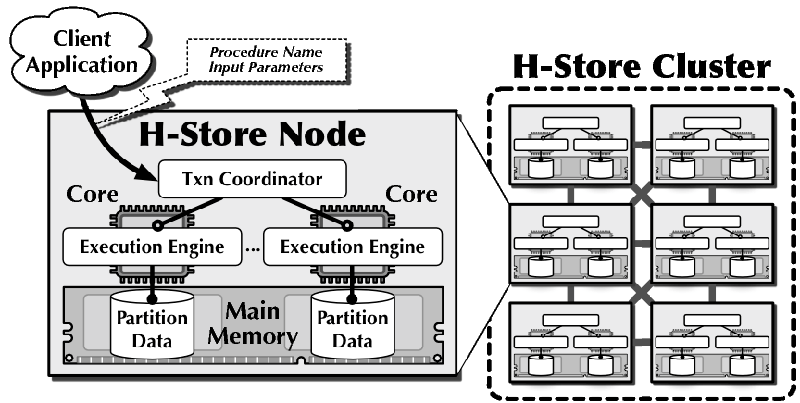
\includegraphics[width=\linewidth]{hstore}}
\caption{H-Store Architecture} \cite{www-H-StoreArch}
\label{fig:false-color}
\end{figure}

H-Store is a parallel, row-storage relational DBMS that runs on a cluster of shared-nothing, main memory executor nodes.

A single H-Store instance is a cluster of two or more computational nodes deployed within the same domain. A node is a single physical computer system that hosts one or more execution sites and one transaction coordinator. A site is the logical operational entity in the system; it is a single-threaded execution engine that manages some portion of the database and is responsible for executing transactions on behalf of its transaction coordinator. The transaction coordinator is responsible for ensuring the serializability of transactions along with the coordinators located at other nodes.A typical H-Store node contains one or more multi-core CPUs, each with multiple hardware threads per core. As such, multiple sites are assigned to nodes independently and do not share any data structures or memory.

Every table in H-Store is horizontally divided into multiple shards that each consist of a disjoint sub-section of the entire table. The boundaries of a table’s fragments are based on the selection of a  column for that table; each tuple is assigned to a fragment based on the hash values of this attribute. H-Store also supports partitioning tables on multiple columns. Related fragments from multiple tables are combined together into a partition that is distinct from all other partitions. Each partition is assigned to exactly one site.

All tuples in H-Store are stored in main memory on each node; the system never needs to access a disk in order to execute a query.It replicates partitions to ensure both data durability and availability in the event of a node failure. Data replication in H-Store occurs in two ways: (1) replicating partitions on multiple nodes and (2) replicating an entire table in all partitions. For the former, H-Store adobts the k-safety concept, where $k$ is defined by the administrator as the number of node failures a database can tolerate before it is deemed unavailable.

Client applications make calls to the H-Store system to execute pre-defined stored procedures. Each procedure is identified by a unique name and consists of user-written Java control code intermixed with parameterized SQL commands. The input parameters to the stored procedure can be scalar or array values, and queries can be executed multiple times.

Each instance of a stored procedure executing in response to a client request is called a transaction. Similarly as with tables, stored procedures in H-Store are assigned a partitioning attribute of one or more input parameters. When a new request arrives at a node, the transaction coordinator hashes the value of the procedure’s partitioning parameter and routes the transaction request to the site with the same id as the hash. Once the request arrives at the proper site, the system invokes the procedure’s Java control code, which will use the H-Store API to queue one or more queries in a batch. The control code invokes another command in H-Store to block the transaction while the execution engine executes the batched queries.

All of operations within a transaction are atomic across all the partitions involved in the transaction. When a transaction executes, it has exclusive access to the data at the partitions that it locks, therefore all of its operations execute on a consistent view of the database and are isolated from all other transactions (since no other transactions execute concurrently at those partitions). Finally, with snapshots and command logging, the state of the database is completely recoverable and all changes made by transactions are durable \cite{kallman2008} \cite{www-H-StoreArch}.

\section{Documentation}

\begin{itemize}
\renewcommand{\labelitemi}{\scriptsize$\bullet$} 
\item Detailed documentation on H-Store  Deployment , Configuration,Debugging and Development is available at  \cite{www-H-Store}
\item H-Store DBMS is open source and complete source code is available in the  \cite{github-H-Store} github repository. 
\end{itemize}

\section{Licensing and Commercial Use}

A commercial implementation of H-Store is VoltDB.VoltDB was developed for production environments, and thus it is focused on high-performance throughput for single-partition transactions and provides robust handling of failures that are obviously needed for a main memory system. H-Store does not have VoltDB’s tools for managing and maintaining clusters. But because H-Store is a research database (thus does not provide many of the safety guarantees that VoltDB does), this allows H-Store to support additional optimizations, such as speculative execution and arbitrary multi-partition transactions.For example, in VoltDB every transaction is either single-partition or all-partition. That is, any transaction that needs to touch multiple partitions will cause the VoltDB’s transaction coordinator to lock all partitions in the cluster, even if the transaction only needs to touch data at two partitions. However H-Store has a different internal transaction coordination subsystem . For each query batch submitted by a transaction, the heavily optimized H-Store Batch Planner determines what partitions each query needs to access and only dispatches requests to those partitions.H-Store uses VoltDB’s VoltProcedure API, so any stored procedures written for VoltDB should still work in H-Store \cite{www-H-StoreFaq}. 


\section{Use Case}

Big Data is data at rest. Big Data describes data’s volume – petabytes to exabytes - and variety: structured, semi-structured and unstructured data that has the potential to be analyzed for information. Big Data systems facilitate the exploration and analysis of stored, large data sets.
Big data is often created by data that is generated at incredible speeds, such as click-stream data, financial ticker data, log aggregation, or sensor data. Often these events occur thousands to tens of thousands of times per second. The benefits of big data are lost if fresh, fast-moving data from real time sources is dumped into HDFS, an analytic RDBMS, or even flat files, because the ability to act or alert right now, as things are happening, is lost. 

So this data stream which is the source for big data is called Fast Data.For Fast Data we're not measuring volume in the typical gigabytes, terabytes, and petabytes . For Fast Data we are measuring volume in terms of time: the number of megabytes per second, gigabytes per hour, or terabytes per day. So the key difference between Big and Fast Data is Volumne vs Velocity.So to build systems and applications to take advantage of Fast Data  to make real-time, per-event decisions that have direct, immediate impact on business interactions and observations we need a DBMS which  offers high speed transactional ACID performance and the ability to process thousands to millions of discrete incoming events per second is ideal for processing such type of data. Fast data systems operationalize the learning and insights that companies derive from big data.NewSQL systems such as H-Store and VoltDB are ideal for the Fast Data use case \cite{www-FastData}.

Below are four common uses cases for Fast Data 
\begin{itemize}
\renewcommand{\labelitemi}{\scriptsize$\bullet$} 
\item Real-time recommendation engines or hyper-personalization applications that can detect and act on individual customer needs in real-time.For example real-time analysis of subscriber data based on event triggers such as the end of a call, use of the mobile device in a particular location, or a user hitting a data usage threshold. These insights can then used to initiate real-time campaigns and communications, delivered while the customer’s device is still in hand. Timely and relevant offers, improved service response, and proactive updates on billing/usage result in a superior customer experience.
\item Real-time, "down to the last dollar" resource management applications, e.g., bid and order management.Managing advertising transactions at scale requires the ability to process transactions fast enough to align advertising purchases with customer budgets. H-Store high speed processing capabilities has the ability to meet the real-time demands of mobile advertising customers while handling a growing number of transactions – all while keeping client ad budget and actual spend aligned.
\item Per-event analytics with automated decision making to enforce a policy or authorization level, e.g., credit card fraud, managing API calls and authorizations in real time.For example we can apply bank business rules to a stream of card swipes, hundreds to thousands of times per second in real time. Using stored procedures to manage the analytic logic, paired with state held in the DBMS, banks can increase their ability to detect fraudulent cards on the first swipe. As blacklists and rules change, these can be uploaded into DBMS , where the new rules and stored procedures immediately affect card processing decisions.
\item Sensor data management in Internet of Things (IoT) applications.For example high-velocity data can be used by utilities to generate insights on a per-event basis. Leveraging the smart energy data, it can alert utilities if their usage is trending toward exceeding their forecasted energy budget.Additionally, reporting meters can be automatically compared to identify meters that did not provide a current status. If a meter misses a defined number of consecutive reporting intervals, a technician can be automatically assigned to fix or replace it.
\end{itemize}

\section{Conclusion}
H-Store and its commercial implementation VoltDB are main memory DBMS designed for applications running on a cluster of nodes needing high transaction throughput. They are ideally suited for the Fast Data use case of Big Data. As an example of a ”NewSQL” DBMS, we
can expect them and other similar main memory Data bases to gradually take over the Modern Transaction Processing market from legacy disk-oriented vendors
because of superior performance.

\section*{Acknowledgements}

The authors thank Prof. Gregor von Laszewski for his technical guidance.
% Bibliography

\bibliography{references}


\end{document}
